\documentclass[a4paper,12pt]{article}

%Dies löst einige Probleme mit der Deutschen Schreibweise
\setlength{\parindent}{0pt}
\setlength{\parskip}{5pt}
%löst Probleme mit ä,ö,ü
\usepackage[utf8]{inputenc}
%\usepackage[T1]{fontenc}
%Deutsche Silbentrennung
\usepackage[ngerman]{babel}

% Grafikpaket laden
\usepackage{graphicx}

%Farbpacket laden
\usepackage{xcolor}

\pagestyle{headings}


\begin{document}

\thispagestyle{empty}
\begin{center}
\Large{Hochschule für Technik Rapperswil HSR}\\
\end{center}

\begin{center}
\Large{MRU: Sensors, Actors and Communication}
\end{center}
\begin{verbatim}







\end{verbatim}
\begin{center}
\textbf{\LARGE{Studienarbeit}}
\end{center}
\begin{verbatim}


\end{verbatim}
\begin{center}
\textbf{\Huge{Yolo auf Fingern}}
\end{center}
\begin{verbatim}



\end{verbatim}
\begin{center}
\textbf{im Studiengang Industrial Technologies}
\end{center}
\begin{verbatim}







\end{verbatim}

\begin{flushleft}
\begin{tabular}{lll}
\textbf{eingereicht von:} & & Heinz Hofmann \flq{}hhofmann@hsr.ch\frq{}\\
& & \\
& & \\
\textbf{eingereicht am:} & & 9. Februar 2017\\
& & \\
& & \\
\textbf{Betreuer/Betreuerin:} & & Herr Prof. Dr. G. Schuster \\
& & Frau T. Mendez
\end{tabular}
\end{flushleft}









\newpage
%Inhaltsverzeichnis
\tableofcontents
% das Abbildungsverzeichnis
\listoffigures

\newpage
%Kapitelüberschrift
\section{Abstract}
\subsection{Aufgabenstellung}
Die Aufgabenstellung in dieser Projektarbeit ist...
%TODO hier weiterschreiben
\subsection{Vorgehen}
\subsection{Fazit}



\newpage
\section{Beispielkapitel}
Dies ist ein weiterer Satz

Wir machen hier weiter mit folgender Fussnote\footnote{\label{foot:nonce1}Damit wird die entsprechende Fussnote beschrieben.}.
Natürlich können viele verschiedene Sätze ensprechende Fussnoten\footnote{\label{foot:nonce2}Auf jeden Fall funktioniert das..} haben.

Ich möchte aber auch auf entsprechen die \ref{foot:nonce1}. Fussnote auf Seite \pageref{foot:nonce1} verweisen.

Auf jedem Fall wird dieser Punkt im Kapitel \ref{subsec:Motivation} auf Seite \pageref{sec:Einleitung} beschrieben.

\subsection{Motivation}
\label{subsec:Motivation}
\subsubsection{Stand der Technik}
\label{subsubsec:Stand der Technik}
Dies ist ein Satz.
Dies ist Satz Nr. 2
Jeder Satz kommt auf eine eigene Zeile.
Soll ein Absatz gemacht werden, muss eine Leerzeile eingefügt werden.
\begin{figure}
	\centering
	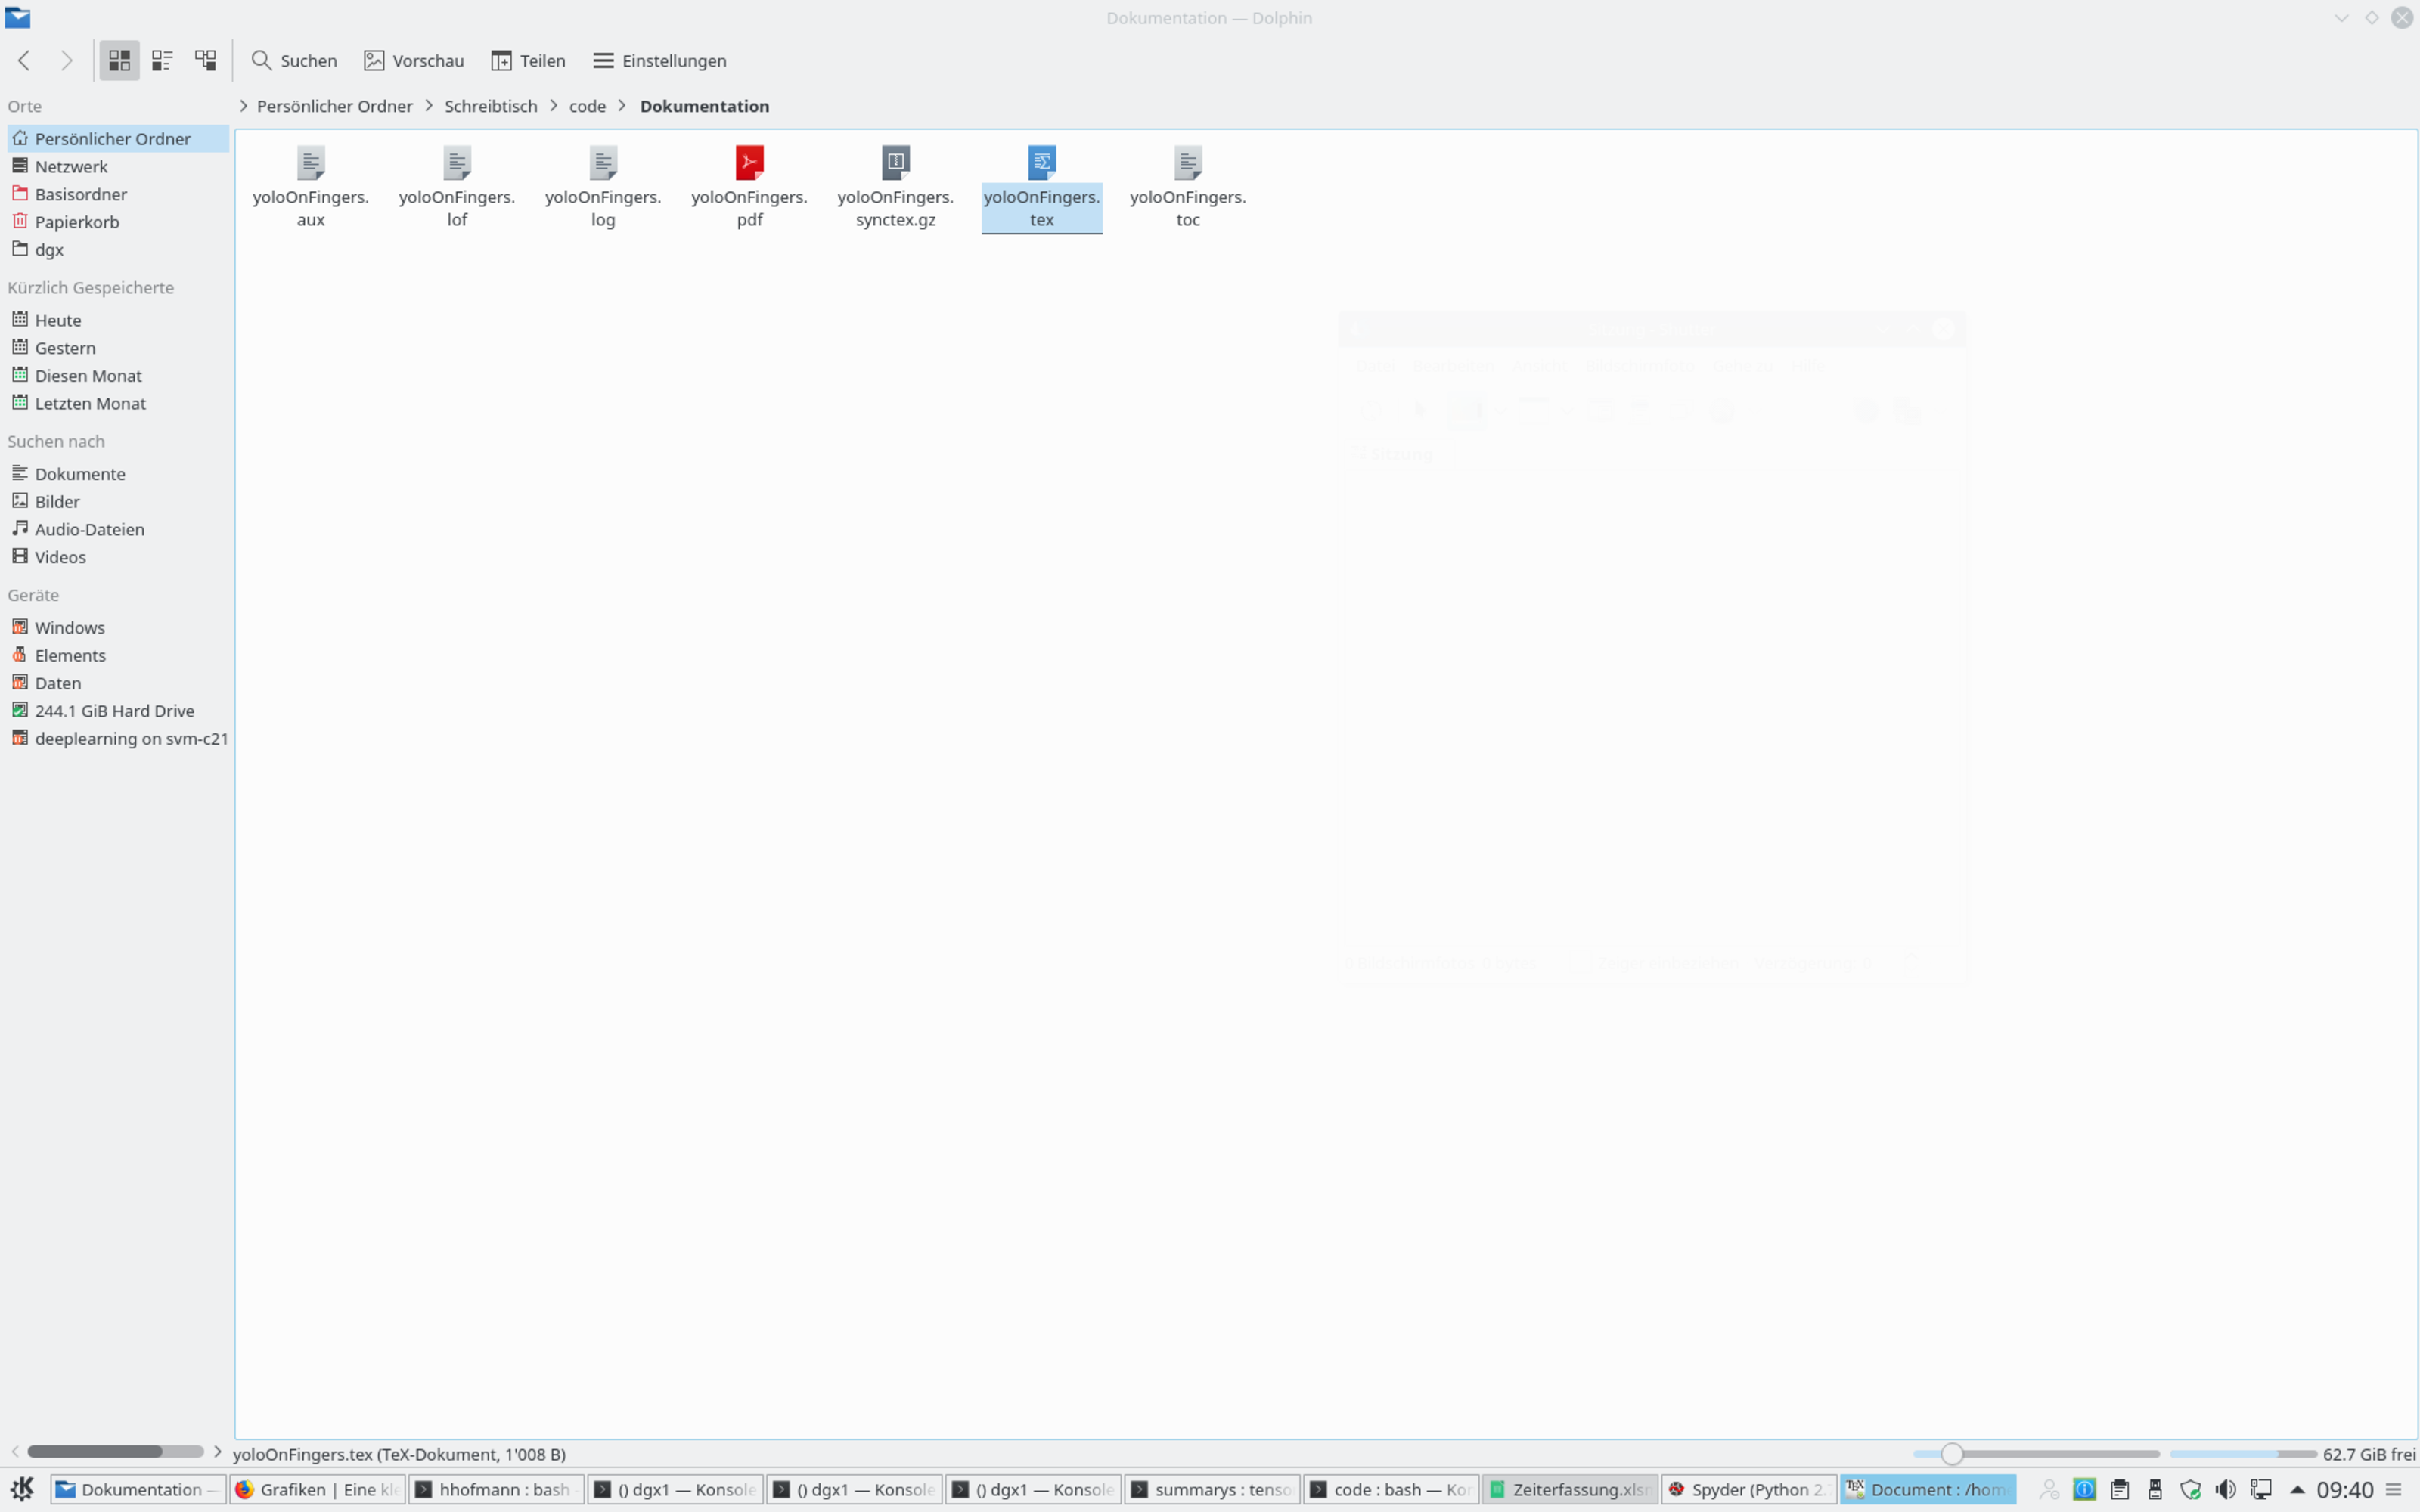
\includegraphics[scale=0.25]{BilderEinleitung/bild.pdf}
	\caption{Dies ist eine Grafik als png}
	\label{img:grafik-dummy1}
\end{figure}

Dies ist Satz Nr.3
Aber jetzt habe ich eine komische einrückung beim Satzstart...?
Naja, da werden wir sicher auch noch herausfinden, warum dies so ist.
\begin{figure}
	\centering
	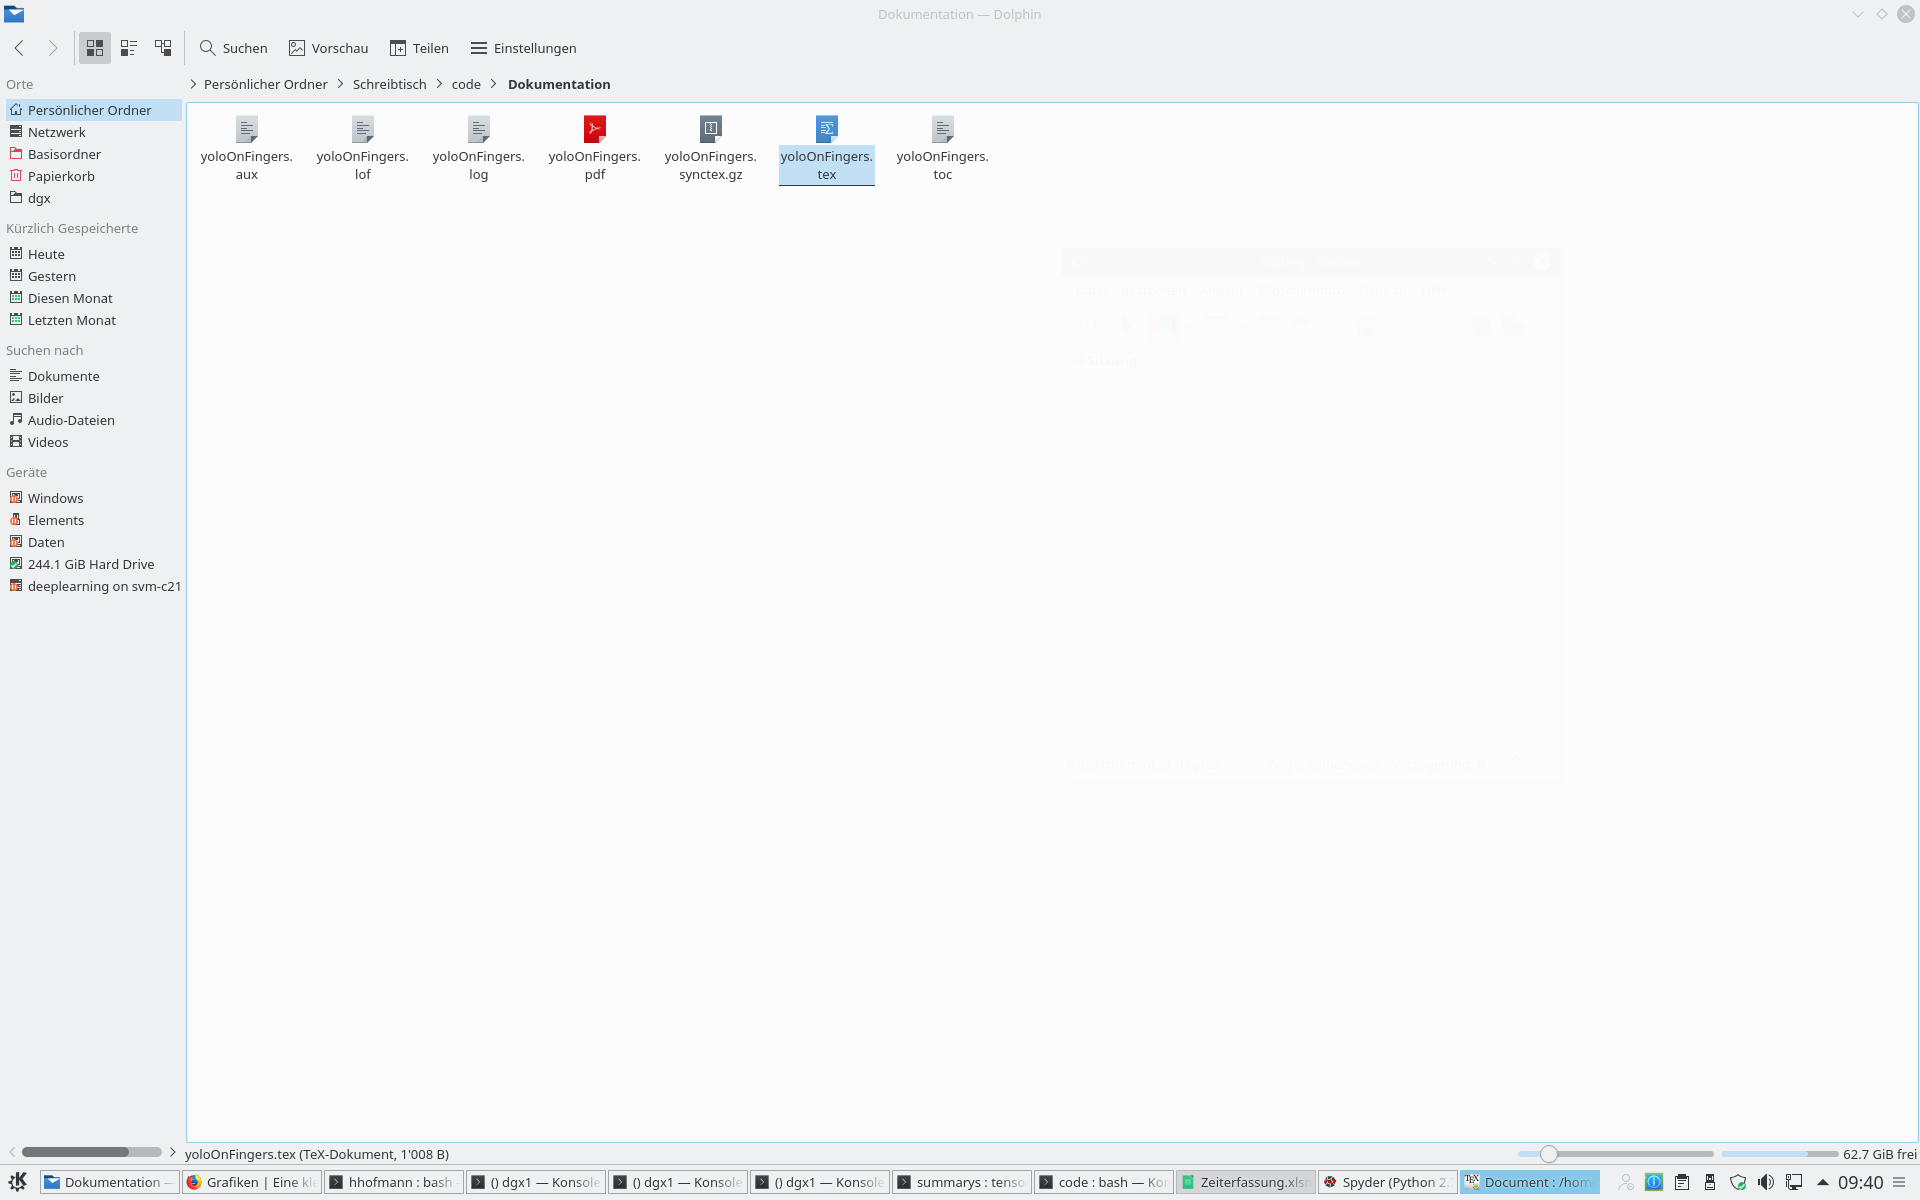
\includegraphics[scale=0.2]{BilderEinleitung/bild.png}
	\caption{Dies ist eine Grafik als pdf}
	\label{img:grafik-dummy2}
\end{figure}
	

So sollte alles auf git schön anzusehen sein...

Weiterhin wollen wir an dieser Stelle Bezug auf die Grafik
\ref{img:grafik-dummy1} auf Seite \pageref{img:grafik-dummy1} nehmen, was uns

\end{document}
